\xchapter{Latência em sistemas operacionais de tempo real}{}\label{cap2}

Neste capítulo serão apresentados as causas de latência em um Sistema Operacional de Propósito Geral e os mecanismos utilizados para tornar estes sistemas em sistemas operacionais de tempo real, assim como será apresentado Linux e as maneiras como o mesmo trata interrupções e os tipos de mecanismos para tal.

\section{Linux}

O Linux é um sistema operacional de propósito geral de código aberto criado por Linus Torvalds em 1991 \cite{LinuxRelease}. Seu modelo de licença e desenvolvimento fez do Linux o projeto de código aberto com uma das maiores comunidades de desenvolvedores. Em 2000, a Linux Foundation, uma organização sem fins lucrativos para promover o crescimento do Linux, foi fundada. Várias empresas fazem parte da Linux Foundation e também estão colaborando com o projeto, incluindo, entre outras, empresas como Google, Cisco, Intel, IBM, Oracle e, mais recentemente, a Microsoft \cite{LinuxFoundation}. 

Hoje o Linux é um dos sistemas operacionais mais populares em sistemas embarcados de prateleira, além de ser a base para o Android, outro sistema bastante popular. Como várias aplicações estão desenvolvidas para o Linux, é importante estudar o seu comportamento e suas garantias temporais. Para isso, veremos como o Linux implementa as interrupções e como as mesmas são capazes de garantir a restrições temporais.

\section{Interrupções}

Os computadores modernos precisam executar várias atividades ao mesmo tempo e também verificar estímulos externos. Ao digitar no teclado, espera-se que o caractere seja exibido na tela imediatamente. Para isso, o processador poderia verificar frequentemente se há alguma tecla pressionada. Uma varredura (\textit{polling}) com frequência baixa poderia tornar a latência de entrada bastante imprevisível e possivelmente longa, enquanto uma varredura com frequência alta levaria o processador a desperdiçar seus ciclos de trabalho, para verificar a existência de eventos externos que podem não ter acontecido \cite{Rothberg2015}. Para evitar esse desperdício de recursos, o processador delega algumas atividades para outros hardware, como controladores USB. Para se comunicar, esses hardwares se baseiam no conceito de interrupções. Essas interrupções são gerenciadas por um hardware específico, o PIC ou o APIC (\textit{Advanced Programmable Interrupt Controller}) que é diretamente conectado ao processador. Quando um dispositivo precisa enviar uma informação ao processador, ele envia um sinal para o APIC que envia o sinal para o processador. Estes eventos de interrupções podem ser gerados também por motivos relacionados a falhas na alimentação, divisão por zero ou outros eventos que podem comprometer o funcionamento do sistema. Os temporizadores também utilizam esse mecanismo para sinalizar o processador.

Os sistemas operacionais têm três casos de uso para tratadores de interrupção. Primeiro, quando uma aplicação faz uma chamada de sistema, ele precisa alternar do espaço do usuário para o espaço do kernel de maneira segura. Segundo, quando ocorre um erro em tempo de execução, como acesso ilegal à memória, que precisa de uma rotina para lidar com esse erro e decidir como proceder ou se o programa deve ser encerrado. Esses dois casos são chamados de interrupções síncronas ou interrupção de software, pois ocorrem em momentos específicos. E, finalmente, quando o hardware externo envia um comando assíncrono para o processador, conforme explicado anteriormente, que é chamado de interrupção assíncrona ou interrupção do hardware \cite{LinuxInterrupts}.

Quando o processador recebe uma interrupção, interrompe o trabalho e transfere o controle para uma função instalada anteriormente para lidar com esse evento. Quando esse evento é tratado, o processador retoma o trabalho que foi interrompido. Assim, qualquer programa comum pode ser interrompido em praticamente qualquer ponto, pois o tratamento de interrupções tem prioridade \cite{LinuxDeviceDrivers}. Enquanto o tratamento de uma interrupção estiver ocorrendo, novas interrupções podem ocorrer. Isso tem o potencial de fazer com que uma interrupção nunca seja tratada ou que nunca execute o programa novamente. Para evitar isso, o kernel é capaz de mascarar interrupções, ou seja, ele pode adiar o tratamento de uma interrupção enquanto outro tratamento já está sendo realizado e, após terminar o primeiro tratamento, tratar as novas interrupções.

\section{O modelo de prólogo e epílogo}

Enquanto um tratador de interrupções está em execução, as interrupções são mascaradas e o tratamento é adiado após a conclusão desse tratador. Isso simplifica o código do tratador, pois o mesmo não precisa lidar com casos em que foi interrompido. Além disso, permitir que um tratador seja interrompido pode causar um \textit{loop} de recursão infinito, que em máquinas com memória finita pode causar um estouro de pilha. Portanto, é preferível adiar o tratamento de novas interrupções, mesmo que isso cause possíveis perdas de interrupção quando várias chegarem ao mesmo tempo. Para impedir que essa perda de interrupção ocorra, os tratadores devem ser pequenos. Isso vai contra a essência de algumas interrupções, como ler e gravar no disco, que são tarefas demoradas. No entanto, essas tarefas não precisam ser executadas imediatamente, nem precisam desativar outras interrupções.

Assim, o modelo de prólogo e epílogo oferece uma maneira de contornar essa limitação, quebrando o tratador em duas partes, tratando apenas a parte crítica com as interrupções desativadas e adiando o máximo de trabalho possível para um contexto em que as interrupções são ativadas novamente. No prólogo, a parte crítica do tratador é executada e a as demais partes são tratadas no epílogo, onde as interrupções estão novamente habilitadas. No Linux, eles também são chamados de \textit{top half} e \textit{bottom half} \cite{OReilly}.

Durante a execução do prólogo, as interrupções são mascaradas. Quando o prólogo lida com a parte crítica, ele enfileira a parte não crítica da interrupção a ser executada no epílogo. Durante o epílogo, as interrupções são ativadas novamente e podem ocorrer outras interrupções. Caso ocorreram, o prólogo da nova interrupção será tratado imediatamente e o epílogo será enfileirado e tratado após o tratamento do epílogo da primeira interrupção.

Essa divisão é comum em muitos sistemas operacionais. O Windows tem sua implementação, que é Chamada de \textit{Deferred Procedure Call}, ou Chamada de Procedimentos Deferidos, para enfileirar tarefas de baixa prioridade \cite{InsideMicrosoftWindows}. No Linux, existem 3 tipos de tratamento para o epílogo, que serão detalhados na próxima sessão.

\section{Tipos de epílogo no Linux}

Depois de tratar o prólogo, o Linux tem três maneiras de lidar com o trabalho não crítico que foi atrasado. O mecanismo Softirq é a maneira mais eficiente, mas menos flexível, pois é implementada diretamente no código do kernel. O mecanismo Tasklet é uma extensão do Softirq e é criado sobre ele. É menos eficiente, mas pode ser implementado como um módulo do kernel. E, finalmente, temos o mecanismo Workqueue, que é tratadas no contexto dos processos e não no kernel. Isso os torna muito flexíveis, mas com um custo de ativação ainda maior \cite{OReilly}.

\subsection{Softirq}

Softirqs são mecanismos simples para transferir trabalho de um contexto ininterrompível para um contexto interrompível. Eles estão associados a tarefas de rede, temporizadores e outras tarefas críticas e são a base dos Tasklets discutidos na próxima sessão. Os softirqs são executados assim que o sistema operacional muda do espaço do usuário para o espaço do kernel ou retorna de uma interrupção. Softirqs são especificados em tempo de compilação e não podem ser alocados em tempo de execução. Há um limite para quantos Softirqs podem ser implantados, já que estão em um vetor específico para isso. Atualmente esse limite é de 32 Softirqs. A prioridade de um Softirq é a posição dentro do vetor.

Quando um Softirq é iniciado, ele é executado até concluir a tarefa. Isso significa que ele só pode ser interrompido por outra interrupção. O código que gerencia a execução do Softirq pode ser executado em vários núcleos do processador, portanto, o desenvolvedor é responsável por garantir a sincronização entre os dados. Como não há garantia de que este Softirq tenha um contexto de processo associado, esse tratador não pode dormir e, como o tratador é executado até sua conclusão, é ideal que ele não consuma muito tempo do processador.

Embora outras interrupções sejam tratadas, nenhuma outra tarefa será tratada até que o Softirq seja concluído. Portanto, mesmo se o tratamento de interrupções for rápido, se houver muitos Softirqs pendentes, as tarefas poderão ser adiadas indefinidamente. Para evitar esse comportamento, sempre que um tratador é finalizado, o tempo de duração da tratador da fila Softirqs é verificado. Se este tempo exceder um limite, a iteração na fila será interrompida. Em vez disso, uma thread de kernel dedicada, \textit{ksoftirqd}, é criada para lidar com essas interrupções \cite{OReilly, Rothberg2015}.

\subsection{Tasklet}

Enquanto o Softirq é simplesmente um índice de tarefas a serem executadas, os Tasklets são ponteiros para estruturas que contêm informações semelhantes, mas isso permite que as estruturas sejam alocadas em qualquer lugar do kernel. Isso permite que esses mecanismos de interrupção sejam implementados como módulos do kernel. Também não há restrições quanto ao número de Tasklets que podem ser implantados.

A estrutura do Tasklet consiste basicamente no tratador associado a ela e no argumento passados a ela. Ao chamar um Tasklet, essa estrutura é enfileirada em uma lista encadeada e marcada com um Softirq específico. Existem duas filas de Tasklet, uma de baixa prioridade e outra de alta prioridade. Ao executar esse Softirq, ele itera sobre as listas do Tasklet e chama o tratador específico para cada um. Portanto, os Tasklets estão no mesmo contexto que o Softirqs, sem processo associado e incapazes de serem postos para dormir. Como o Softirqs, eles são executados no processador na qual foram chamados para aumentar a localidade dos dados e melhorar a utilização do cache.

Antes de chamar o tratador de um Tasklet, você deve bloquear sua estrutura. Quando essa estrutura já está bloqueada, esse tratador é colocado na fila novamente e o Softirq que verifica os Tasklets é novamente marcado como pendente. Isso implica que apenas um Tasklet pode ser executado no processador a qualquer momento e simplifica o código necessário além de evitar conflitos de concorrência.

Os Tasklets são mais fáceis de usar e mais flexíveis e podem ser usados em qualquer lugar do kernel. Por serem baseados no Softirq, eles têm as mesmas limitações de não poderem ser postos para dormir. Essa limitação não existe nos Workqueue, que serão tratados a seguir \cite{OReilly, Rothberg2015}.

\subsection{Workqueue}

Os Workqueues são usados quando precisamos tratar uma tarefa fora do contexto de interrupção e essa tarefa dorme ou fica bloqueada. A tarefa a ser executada é encapsulada e enfileirada na fila de Workqueues. Threads dedicadas executam as tarefas nesta fila. Quando essa tarefa precisa dormir ou ser bloqueada, o escalonador de tarefas do sistema operacional pode simplesmente alterar a tarefa a ser executada. Isso aumenta a capacidade de resposta, impedindo que os threads do usuário parem enquanto são tratadas interrupções longas.

Como o comprimento da fila é variável, o número de threads dedicadas à execução dos itens da fila de Workqueues precisa ser dinâmico para evitar desperdício de recursos. Essa fila é primeiro organizada em filas secundárias, pelo menos uma fila de alta prioridade e uma fila de baixa prioridade, cada uma com uma thread dedicada associada. Quando uma fila secundária fica vazia, a thread dedicada é colocada em suspensão. Quando novos itens são adicionados, a thread é acordada para processar esses novos itens. Para evitar desperdiçar memória, quando uma thread gasta muito tempo dormindo, é destruída. No entanto, sempre há pelo menos uma thread em espera para processar interrupções na fila. Por outro lado, quando a fila está crescendo e o uso do processador não é maximizado, novas threads são criadas.

A capacidade de dormir ou ser bloqueada torna os Workqueues muito mais flexíveis do que outros mecanismos. O custo é que essas tarefas são tratadas por threads gerenciados pelo escalonador, tendo um custo para gerenciar. Os Workqueues também podem ser executados em qualquer núcleo, dificultando a obtenção das informações necessárias em cache \cite{OReilly, Rothberg2015}.

\section{Sistemas Operacionais de tempo real}

Entre os desenvolvedores há um ditado que diz \say{um sistema de tempo real é um sistema que faz o que você espera que ele faça no tempo que você espera que ele faça} \cite{LinuxFoundationRT}. Assim, qualquer sistema pode ser considerado um sistema de tempo real desde que exista restrições temporais para os serviços que ele oferece. Por exemplo, um sistema hospitalar que precise medir os batimentos cardíacos de um paciente a cada segundo e avise aos médicos caso ocorra alguma alteração acaba sendo um sistema de tempo real. Ainda que um segundo possa ser considerado um intervalo de tempo longo comparado com o desempenho de sistemas computacionais modernos, é o limite máximo de tempo para que este sistema hospitalar funcione de acordo com a restrição temporal especificada, sob pena de risco a vida humana \cite{Puhlmann2014}. Em alguns casos, a realização da tarefa fora do tempo esperado provoca apenas uma degradação da qualidade do serviço oferecido pela aplicação, mas em outros casos esse atraso pode comprometer toda a operação do sistema. Em um sistema de controle ou segurança, por exemplo, um atraso em uma ação específica, como acionar um alarme ou ativar um controle de incêndio, pode levar a mortes de pessoas. Assim, Burns define um sistema de tempo real como \say{um sistema que processa informação e que tem que responder corretamente a um estímulo gerado externamente dentro de tempo finito e especificado} \cite{Burns2001}.

O tempo entre o início de um evento e o momento em que os seus efeitos se tornam perceptíveis é chamado de latência. Em sistemas complexos, existem diversos tipos de latência que se somam para formar uma latência global. Em um exemplo de uma instrução enviada via rede internet, por uma impressora a um processo cliente, podemos distinguir as seguintes latências entre o instante no qual a impressora emite uma instrução e a execução desta instrução pelo processo cliente destinatário: 

\begin{itemize}
    \item a \textbf{latência de rede} associada ao tipo de conexão de rede e a diversidade de roteadores e switches ao longo do caminho;
    \item a \textbf{latência de interface} associada ao processamento da mensagem na camada de enlace pela placa de rede para identificar o processo destinatário e detectar eventuais erros em redes sem-fio;
    \item a \textbf{latência de interrupção do prólogo} associada ao intervalo de tempo entre o instante no qual a placa de rede gera uma interrupção informando o processo destinatário da existência de uma mensagem pendente a ser recebida e o início do tratamento desta interrupção pelo processador;
    \item a \textbf{latência de execução do prólogo} associada ao tempo de processamento do prólogo;
    \item a \textbf{latência de ativação do epílogo} associada ao intervalo de tempo entre o instante no qual o processador termina a execução do prólogo da interrupção da placa de rede e inicia o processamento do epílogo;
    \item a \textbf{latência de execução do epílogo} associada ao tempo de processamento do epílogo;
    \item a \textbf{latência de escalonamento} associado ao intervalo de tempo entre o termino do serviço de recepção da mensagem e o início da execução da instrução pelo processo destinatário;
    \item a \textbf{latência de processamento} associada ao tempo de processamento da mensagem pelo processo cliente;
\end{itemize}

\begin{figure}[!htb]
    \centering
    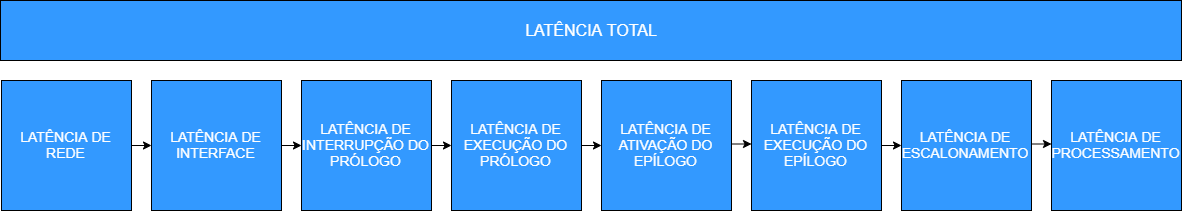
\includegraphics[width=\textwidth]{graficos/latencias.png}
    \caption{Latências envolvidas em uma instrução enviada pela rede}
    \label{flux:latencias}
\end{figure}


A latência de rede é imprevisível pois a quantidade de roteadores e switches na rede pode aumentar e diminuir sem que seja possível prever essa alteração, além de que, mesmo em estruturas que não mudem, as mensagens podem percorrer caminhos diferentes a depender dos buffers e memórias dos roteadores. Numa rede sem fio a latência de interface também é imprevisível pois podem ocorrer retransmissões arbitrariamente devido a erros no recebimento da mensagem. A latência de interrupção do prólogo depende do estado do processador na hora da interrupção do processador pela placa de rede, pois podem existir eventos com prioridade maior ou outras interrupções pendentes provocando um atraso no tratamento deste interrupção, que tornam este tempo imprevisível. A latência de ativação do epílogo tem seu tempo influenciado pela quantidade de processos sendo executados pelo processador além da possibilidade de ocorrência de novas interrupções. A latência de execução do epílogo é imprevisível pois neste momento as interrupção estão novamente habilitadas, então o trotador pode ser interrompido arbitrariamente. A latência de escalonamento é influenciada pelo número de processos em execução no processador e suas respectivas prioridades. E a latência de processamento, que é o tempo necessário para o processo cliente tratar a mensagem. Todas essas latências e suas componentes não previsíveis, tornam a latência global muito difícil, ou mesmo impossível, de se estimar.

Nesse contexto de imprevisibilidade das latências da aplicação a eventos externos, e aplicações que precisam responder dentro de um tempo limite, devido a suas restrições temporais, adaptar um Sistema Operacional de Propósito Geral em um Sistema Operacionais de Tempo Real é um desafio, visto que estes sistemas precisam lidar com aplicações com restrições temporais e aplicações que são do tipo \textit{best effort} e não possuem requisitos temporais. Ambas as classes de aplicações precisam ser executadas ao mesmo tempo e talvez se comunicar entre si com níveis mistos de criticidade \cite{Cartwrigh2018}.

Para este trabalho foram instalados o Preempt-RT e o Xenomai, patches de tempo real para o Linux, no Raspberry Pi. Devido a problemas nos testes com o Xenomai e o INTSight, foi estudado apenas como o Preempt-RT se comporta em relação ao Linux padrão quando se compara a latência de ativação das duas soluções. Foram também realizadas medições para quantificar essa diferença entre eles.